\section{Wykonanie badań metod segmentacji obrazu}
Przeprowadzone przeze mnie badania miały na celu porównanie metod segmentacji obrazu, a także sprawdzenie, jak dobór parametrów dla poszczególnych metod wpływa na jakość uzyskiwanego rezultatu.

\subsection{Narzędzia implementacja algorytmów}
Opisane niżej algorytmy segmentacji obrazu zostały napisane w języku C++ i skompilowane w systemie operacyjnym Linux. Implementacja jest jednak niezależna od systemu operacyjnego, i dzięki uniwersalnemu systemowi budowania CMake, z powodzeniem można w łatwy sposób skompilować i uruchamiać algorytmy pod innymi popularnymi systemami operacyjnymi, takimi jak Windows czy Mac OSX.\\
Ze względu na wykorzystanie w algorytmach segmentacji podstawowych operacji przetwarzania obrazu (takich jak dodawanie obrazu, operacje morfologiczne), zdecydowałem się użyć gotowej biblioteki OpenCV, udostępniającej wiele funkcji pomocnych przy implementacji złożonych algorytmów przetwarzania obrazów.\\
Do rozpoznawania tekstu wykorzystałem bibliotekę Tesseract. Biblioteka Tesseract jest otwartym oprogramowaniem rozwijanym od 1985 roku. Służy do rozpoznawania znaków w obrazach cyfrowych.
\subsection{Aplikacja testująca}
Podczas implementacji algorytmów, bardzo często musiałem zmieniać wartości ich parametrów. Każdorazowe zmiany w kodzie źródłowym i ponowna kompilacja algorytmów była czasochłonna, dlatego napisałem aplikację, która umożliwi mi zmianę parametrów algorytmów bez konieczności zmieniania wartości w kodzie źródłowym, ale podczas działania aplikacji.\\
Następnie do aplikacji dodałem możliwość uruchamiania testów automatycznych, których celem była szybka weryfikacja większej ilości danych testowych na raz, zwracając procentową wartość poprawnie rozpoznanych obrazów. Na rysunku~\ref{fig:tuner_screenshot} zamieszczone zostało okno główne aplikacji testującej.

\begin{figure}
  \centering
  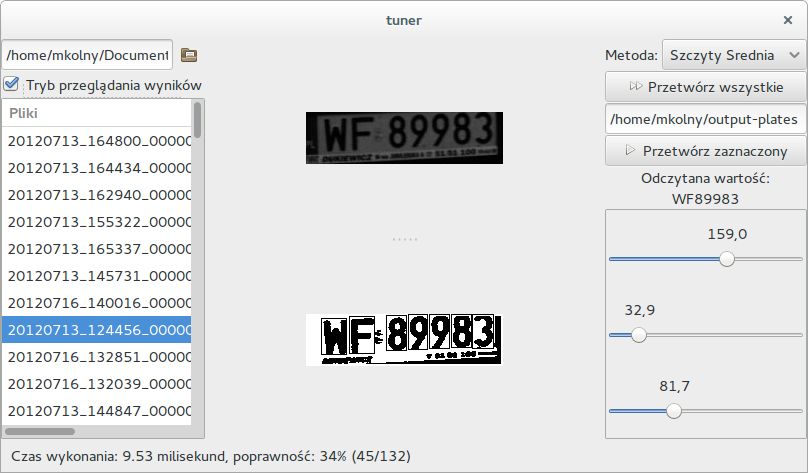
\includegraphics[width=1\textwidth]{img/tuner-screenshot}
  \caption{Widok okna głównego aplikacji do testowania i doboru parametrów algorytmów}
  \label{fig:tuner_screenshot}
\end{figure}
\subsection{Algorytm rozpoznawania znaków na tablicy rejestracyjnej}
Podczas testowania różnych metod segmentacji obrazów, korzystałem zawsze z takiego algorytmu. Schemat blokowy tego algorytmu został przedstawiony na rysunku~\ref{fig:main_flowchart}. Poniżej omówiłem poszczególne bloki schematu.
\begin{enumerate}
  \item \textbf{Konwersja do skali szarości}\\
    Wszystkie operacje, jakich używam w swoim programie, wykorzystują obrazy w skali szarości, dlatego pierwszą czynnością, jaką wykonuje program, jest zmiana obrazu wejściowego na obraz monochromatyczny (jeśli zachodzi taka potrzeba).
  \item \textbf{Wyrównanie histogramu}\\
    Wyrównanie histogramu poprawia kontrast w obrazie, dzięki czemu różnice jasności pomiędzy tłem i znakami są wyraźniejsze, dzięki temu kolejne operacje mogą operować na szerszym zakresie wartości jasności.
  \item \textbf{Detekcja jasności tła i odwrócenie kolorów} \\
    Wszystkie metody segmentacji jakich użyłem zakładają, że tło obrazu jest jaśniejsze od znaków. Dlatego przed wykonywaniem operacji segmentacji następuje detekcja jasności tła, i jeśli zachodzi taka potrzeba, odwrócenie kolorów. Metodę użytą w tej operacji opisałem szczegółowo w akapicie~\ref{ssec:different_backgrounds}.
  \item \textbf{Preprocessing}\\
    Prawie każda metoda segmentacji wymaga wcześniejszego przygotowania obrazu w taki sposób, aby rezultaty były jak najlepsze. W niektórych przypadkach jest to rozmycie obrazu, dla innych metod są to operacje morfologiczne czy operacje działające na histogramie obrazu (np. wyrównanie histogramu).
  \item \textbf{Segmentacja obrazu}\\
    Blok ten reprezentuje implementację jednej metody segmentacji obrazu. Wszystkie badane metody segmentacji obrazu zostały wymienione i opisane w dalszej części tego rozdziału.
    \item \textbf{Określenie warunków poprawnych segmentów}\\
      Na podstawie wyników segmentacji algorytm definiuje kryteria, jakie powinien spełnić segment, aby zostać sklasyfikowany jako znak. Metody określania warunków zostały opisane w podpunkcie~\ref{ssec:different_formats} i~\ref{ssec:additional_elements}.
    \item \textbf{Odrzucenie niepoprawnych segmentów}\\
      Na tym etapie algorytm sprawdza wszystkie warunki określone w poprzednim punkcie, i usuwa ze zbioru segmentów te, które nie spełniają określonych wcześniej kryteriów.
    \item \textbf{OCR}\\
      Obraz jest kadrowany dla każdego segmentu osobno. Seria wykadrowanych obrazów przekazywana jest do algorytmu rozpoznawania znaków, którego zadaniem jest zwrócenie jednej wartości znaku, który zapisany jest w obrazie.
    \item \textbf{Weryfikacja poprawności}\\
      Ostatni etap nie jest już elementem algorytmu rozpoznawania tablic rejestracyjnych, ale jest on użyty w mojej aplikacji w celu weryfikacji poprawności operacji segmentacji oraz rozpoznawania znaków. Program sprawdza, czy ciąg znaków zwrócony w poprzednim podpunkcie jest taki sam, jak oczekiwany. Wartości oczekiwane wyznaczane były przez człowieka patrzącego na obraz.
\end{enumerate}
Poszczególne uruchomienia wyróżniały się tylko implementacją bloków \textbf{preprocessing} oraz \textbf{segmentacja obrazu}.
\begin{figure}
  \centering
  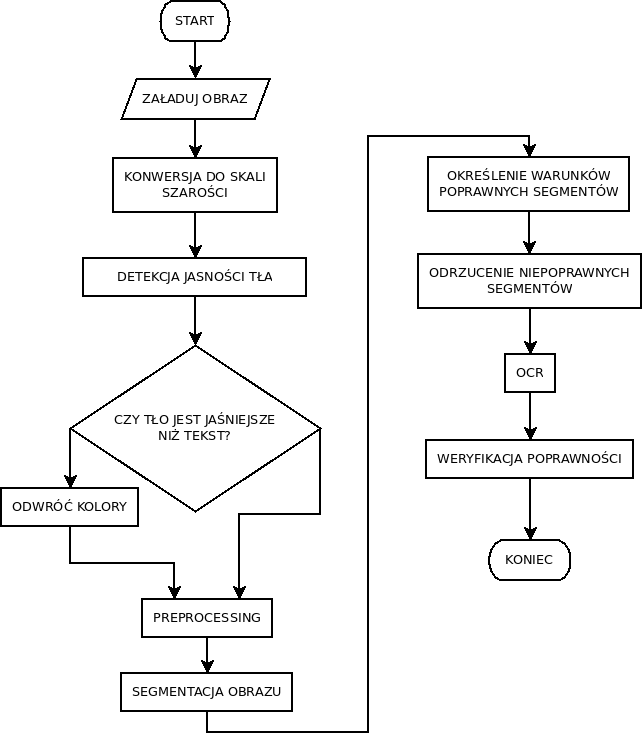
\includegraphics[width=0.98\textwidth]{img/main-flowchart}
  \caption{Schemat blokowy algorytmu rozpoznawania tablic rejestracyjnych}
  \label{fig:main_flowchart}
\end{figure}

\subsection{Porównywane metody segmentacji obrazu}
Poniżej wymieniłem oraz scharakteryzowałem metody segmentacji, które porównywałem na zestawie obrazów tablic rejestracyjnych. Ponadto omówiłem też metody wstępnego przetwarzania obrazu, które dla danej metody segmentacji poprawiają rezultaty. Przedstawiłem też parametry poszczególnych metod, jakie mogą wpływać na działanie algorytmu.

\textbf{Wyszukiwanie szczytów histogramu}\\
Zauważyłem, że metoda wyszukiwania szczytów histogramu zwraca o wiele lepsze wyniki, kiedy przed wykonaniem procesu wyszukiwania szczytów w histogramie, obraz zostanie wyostrzony. Operacja wyostrzenia spowoduje zniknięcie rozmytych krawędzi, dzięki czemu szczyty histogramów będą jednoznaczne. \\
Parametrem dodatkowym algorytmu jest minimalna odległość od wartości szczytowych w histogramie. Przeprowadziłem badania dla różnych wartości minimalnej odległości.\\

